\documentclass[a4paper,10pt]{article}
\usepackage[utf8]{inputenc}
\usepackage{float}
\usepackage{graphicx}
\graphicspath{ {../files/} }

\begin{document}
	
	\title{Rechnernetze - Belegdokumentation}
	\author{Jonathan Vincent Cremer}
	
	\maketitle
	
	\section{Aufgabenstellung}
	Ziel dieser Belegarbeit war es "ein Programm (client + server) zur Übertragung beliebiger Dateien zwischen zwei Rechnern, basierend auf dem UDP-Protokoll" zu erstellen. Als Programmiersprache war JAVA vorgegeben. Das Stop-and-Wait-Protokoll sollte implementiert werden.
	
	\section{Funktionsweise}
	\subsection{Client}
	Die Clientklasse erwartet drei Argumente: Host, PortNr, Datei. Zunächst wird geprüft, ob die Argumentenliste vollständig ist.
	Es wird geprüft, ob der Pfad/Dateiname, der als Parameter übergeben wurde, existiert. Andernfalls beendet sich der Client. Als Maximum Transmission Unit (MTU) sind 1500 Bytes gewählt. 
	Vor der Übertragung wird die Anzahl der zu übertragenden Pakete berechnet, sowie die letzte und vorletzte Paketgröße. Dies ist notwendig, da alle anderen Pakete mit einer Anzahl von 1497 Informationsbytes versendet werden. Der CRC-Code soll im letzten Paket komplett versendet werden. Daher ist eine Größenberechnung des vorletzten Pakets notwendig.
	Der Client speichert die aktuelle Systemzeit um später	 Übertragungsinformationen mitteilen zu können.
	Der Client durchläuft eine Schleife bis alle Pakete erfolgreich übertragen werden. 
	
	Bis zur ersten erfolgreichen Übertragung wird das zu sendende Paket mit den Startpaket-Informationen(nach gegebenem Protokoll) gefüllt. Anschließend  erfolgt die Übertragung der Datenpakete.
	
	Am Ende der Schleife versendet der Client das Paket. 
	Der Client startet eienen Timer. Sofern nach 1000ms (statisch gewähltes timeout) keine Antwort vom Server eintrifft, wird das Paket erneut versendet.
	Sollte die Antwort rechtzeitig eintreffen, wird geprüft, ob das erhaltene ACK mit dem versendeten ACK übereinstimmt. Sofern dies der Fall ist, wird der Erfolgszähler (Anzahl an erfolgreichen Paketübertragungen) um eins nach oben gezählt. Andernfalls versendet der Client dasselbe Paket erneut und setzt den Timeout-Timer zurück. Falls ein Timeout zehn mal hintereinander auftritt, wird das Programm beendet.
	
	\begin{figure}[H]
		\caption{Zustandsdiagramm - Client}
		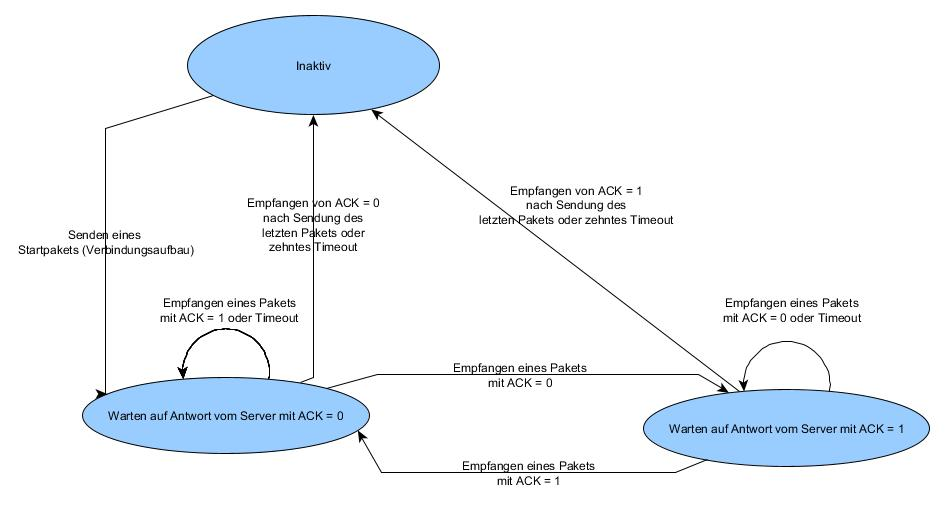
\includegraphics[width=\linewidth]{Zustandsdia_Client.jpg}
		\label{fig:Client}
	\end{figure}

	\subsection{Server}
	Dem Server wird der Port, auf dem er lauschen soll, als Parameter übergeben. Er wartet auf die Ankuft eines Pakets. Sobald das erste Paket ankommt, prüft er, ob es die Kennung "Start" an festgelegter Position enthält. Ist dies nicht der Fall, beendet sich der Server. Es wird geprüft, ob der enthaltene CRC-Code über das Startpaket gültig sein kann.	Nun liest der Server den erhaltenen Pfad/Dateinamen und modifiziert diesen, falls dieser im aktuellen Verzeichnis schon vorhanden sein sollte.
	Der Server liest nun die erhaltenen Datenpakete. Stimmt die erhaltene Paketnummer mit dem erwarteten ACKs überein, handelt es sich um ein neues Paket. Dessen Informationsbits werden ausgelesen und in die zu Beginn erstellte Datei geschrieben. Der Wert des erwarteten ACK wird um 1 (mod 2) erhöht. Gibt es keine Übereinstimmung, so sendet der Server ein Paket mit der zuletzt erhaltenen (validen) Paketnummer an den Client. Sobald alle Pakete übertragen wurden, überprüft der Server den erhaltenen CRC-Code über die Datei auf Gültigkeit. Anschließend wird dessen Ergebnis sowie einige Übertragungsinformationen ausgegeben und der Server beendet sich.
	


	\begin{figure}[H]
		\caption{Zustandsdiagramm - Server}
		\centering
		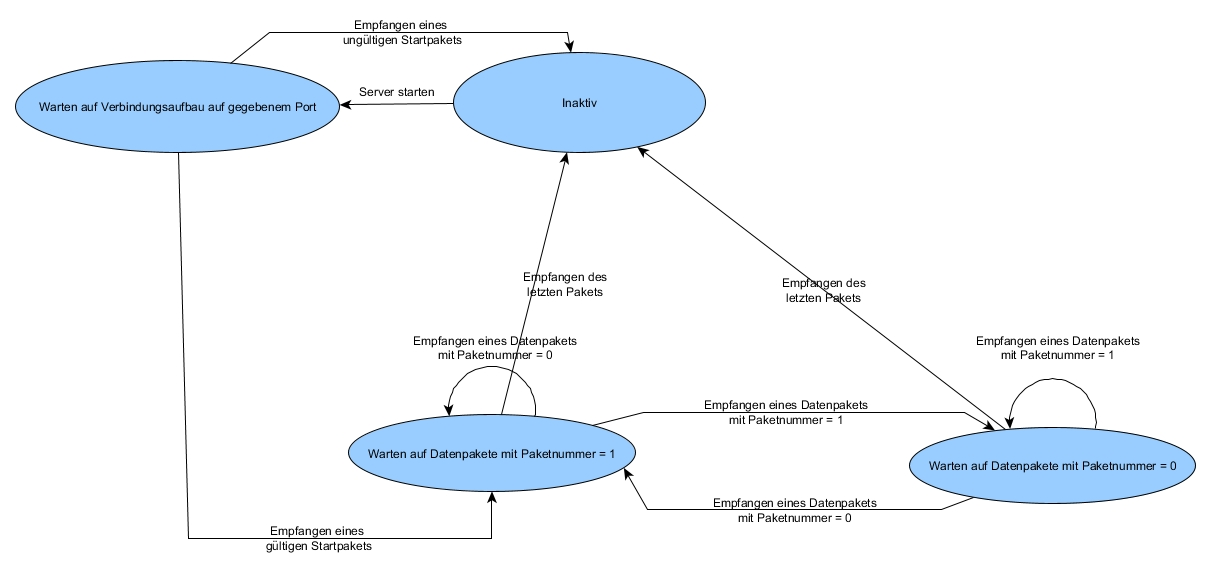
\includegraphics[width=\linewidth]{Zustandsdia_Server.jpg}
		\label{fig:Server}
	\end{figure}

	\begin{equation}
		\label{simple_equation}
		\alpha = \sqrt{ \beta }
	\end{equation}
	
	
	\section{Protokollbewertung}
		
	\subsection{Probleme}
	Ein Problem dieses Protokolls ist, dass das letzte ACK des Servers möglicherweise nicht angekommen ist, der Server dieses allerdings nicht erneut sendet, da er keine weiteren Pakete mehr erwartet. Somit kann der Client nicht feststellen, ob das letzte Paket angekommen ist.
	
	\subsection{Limitierungen}
	Die Datenrate bei diesem Protokoll verhält verhältnismäßig gering aus, da der Client mindestens eine ganze RTT (RTT * AnzahlVersucheBisErfolg) abwarten muss, bis er ein neues Paket lossenden kann. Außerdem wurde in diesem Fall keine Fehlerkorrektur implementiert. Fehlerhafte Pakete verursacht somit eine deutliche Verschlechterung der Datenrate.
	
	\subsection{Verbesserungsvorschläge}
	Besser wäre es, wenn die ACKs nicht binär wären und Der Client nicht auf die Antwort des Servers warten würde, sondern unmittelbar weitere Pakete losschickt in der Hoffung, dass die Übertragung fehlerfrei erfolgt. Im Fehlerfall springt der Client an jene Stelle zurück, an welcher der Server die Pakete als angekommen gemeldet hat. Denkbar wäre im Falle häufiger Paketverluste das doppelte Senden von identischen Paketen, sodass die Chance eines Verlustes halbiert wird.
	
	\section{Performance}
	
	max.erzielbaren Durchsatz bei 10\% Paketverlust und 10 ms Verzögerung für ein einzelnes Paket:
	\begin{equation}
		\label{simple_equation}
		\eta_{sw} = 
		\frac{T_{p}}{T_{p}+T_{\omega}}(1-P_{de})(1-P_{rü})R
	\end{equation}
	\begin{equation}	
		geg: T_{a} = 10ms, P_{de} = P_{rü} = 0.1, 
		R = 1497/1500 = 0,998
	\end{equation}
	Verbindungsgeschwindigkeit in meinem Lan: 135 MB/ S
	\begin{equation}	
		T_{p} = \frac{150B*s}{135000000B} = 0.000001 s = 0,001 ms
	\end{equation}
		\begin{equation}	
		T_{ACK} = 3B*S / 135000000B = 0,0002 ms
		\end{equation}
	\begin{equation}	
		T_{\omega} =  2 * T_{a} + T_{ACK}  \approx 20ms,
	\end{equation}


	\begin{equation}
	\label{simple_equation}
	\eta_{sw} = 
	\frac{0,001}{0,001+20}(0.9)(0.9)0.998 = 0,00004 = 0,004\%
	\end{equation}
	Der niedrige Durchsatz kommt dadurch zustande, dass nur eine sehr geringe Menge an Bytes gesendet wird und auf dessen Antwort gewartet werden muss. 
	In der Praxis wird die Übertragungsverzögerung niedriger sein und zwar  aufgrund der Verwaltungskosten, also Startpaket, Validitätsprüfung, Speicherzugriffe..
	
	Ergebnis für ein in der Praxis zufällig gewähltes einziges Paket:
	\begin{equation}	
	T_{\omega} + T_{P} =  39ms, Annahme: T_{\omega} = 20ms
	=> \eta_{sw} = 39,4\%
	\end{equation}
	
	
\end{document}